\documentclass[12pt,a4paper]{article}
\usepackage[margin=2.4cm,top=2.6cm,bottom=2.5cm]{geometry}
\usepackage{fontspec}
\usepackage{graphicx}
\usepackage{xcolor}
\usepackage{booktabs}
\usepackage{tabularx}
\usepackage{array}
\usepackage{enumitem}
\usepackage{fvextra}
\usepackage{float}
\usepackage{caption}
\usepackage{fancyhdr}
\usepackage{hyperref}
\usepackage{setspace}
\setmainfont{Times New Roman}
\setsansfont{Arial}
\setmonofont{Consolas}
\graphicspath{{figures/}}
\definecolor{deepblue}{HTML}{17243C}
\definecolor{accentblue}{HTML}{315FCE}
\hypersetup{colorlinks=true,linkcolor=deepblue,urlcolor=accentblue,
  pdftitle={Báo cáo bài thực hành ứng dụng di động - Danh sách sản phẩm},
  pdfauthor={Đông Đức Nguyên}}
\captionsetup{font=small,labelfont=bf}
\setlist[itemize]{leftmargin=1.5em,itemsep=3pt,topsep=4pt}
\setlist[enumerate]{leftmargin=1.7em,itemsep=3pt,topsep=4pt}
\setstretch{1.18}
\setlength{\parindent}{1.2cm}
\setlength{\parskip}{3pt}
\emergencystretch=3em
\renewcommand{\contentsname}{Mục lục}
\renewcommand{\figurename}{Hình}
\renewcommand{\tablename}{Bảng}
\newcommand{\codepath}[1]{\nolinkurl{#1}}
\newcommand{\codecaption}[1]{\par\noindent\textbf{Đoạn mã:} #1\par\vspace{3pt}}
\pagestyle{fancy}
\fancyhf{}
\fancyhead[L]{\small Báo cáo bài thực hành ứng dụng di động}
\fancyhead[R]{\small B23DCVT311}
\fancyfoot[C]{\thepage}
\renewcommand{\headrulewidth}{0.4pt}
\setlength{\headheight}{15pt}

\begin{document}
\hypersetup{pageanchor=false}
\begin{titlepage}
\centering
\vspace*{1.4cm}
{\Large\bfseries BÁO CÁO BÀI THỰC HÀNH\par}
\vspace{0.35cm}
{\Large LẬP TRÌNH ỨNG DỤNG DI ĐỘNG\par}
\vspace{1.6cm}
{\color{accentblue}\rule{0.82\textwidth}{1.2pt}\par}
\vspace{0.45cm}
{\Huge\bfseries ỨNG DỤNG DANH SÁCH SẢN PHẨM\par}
\vspace{0.45cm}
{\large Kotlin -- Android -- JSON Assets\par}
\vspace{0.45cm}
{\color{accentblue}\rule{0.82\textwidth}{1.2pt}\par}
\vspace{2.2cm}
\begin{tabular}{rl}
\textbf{Sinh viên thực hiện:} & ĐÔNG ĐỨC NGUYÊN\\[0.25cm]
\textbf{Mã sinh viên:} & B23DCVT311\\[0.25cm]
\textbf{Nội dung:} & Danh sách, lọc, tìm kiếm và chi tiết sản phẩm
\end{tabular}
\vfill
{\large Ngày 02 tháng 10 năm 2026\par}
\end{titlepage}

\pagenumbering{roman}
\hypersetup{pageanchor=true}
\section*{Tóm tắt}
Bài thực hành xây dựng một ứng dụng Android bằng Kotlin để trình bày danh mục sản phẩm.
Dữ liệu gồm 30 sản phẩm thuộc 6 danh mục, được đọc trực tiếp từ tệp
\codepath{app/src/main/assets/database.json}; ảnh chụp sản phẩm đại diện được đóng gói cùng ứng dụng.
Màn hình thứ nhất hiển thị danh sách bằng \texttt{ListView}, \texttt{ArrayList<Product>}
và \texttt{ArrayAdapter<Product>}; hỗ trợ lọc theo danh mục và tìm kiếm theo tên hoặc mã.
Màn hình thứ hai hiển thị thông tin chi tiết của sản phẩm được chọn.
Báo cáo trình bày yêu cầu, thiết kế, mã nguồn chính, ảnh chụp màn hình và kết quả kiểm tra.
\tableofcontents
\clearpage
\pagenumbering{arabic}

\section{Tổng quan bài thực hành}
\subsection{Bối cảnh và mục tiêu}
Mục tiêu của bài thực hành là kết hợp đọc dữ liệu JSON cục bộ với các thành phần giao diện
Android cơ bản. Ứng dụng cần đưa dữ liệu từ tệp vào mô hình Kotlin, chuyển mô hình thành
các hàng của danh sách, xử lý thao tác lọc và tìm kiếm, rồi mở một Activity khác để xem chi tiết.
Đây là quy trình đầy đủ từ dữ liệu đến giao diện và điều hướng.

\subsection{Yêu cầu chức năng}
\begin{enumerate}
\item Tạo tệp \codepath{database.json} chứa khoảng 30 bản ghi. Mỗi bản ghi có
\texttt{code}, \texttt{name}, \texttt{price}, \texttt{category}, \texttt{image}
và \texttt{description}.
\item Tạo \texttt{ArrayList<Product>}, lớp \texttt{ArrayAdapter<Product>} và
gán adapter cho \texttt{ListView} bằng \texttt{setAdapter}.
\item Trên màn hình danh sách, hiển thị tên và mã sinh viên, tiêu đề
“Danh sách sản phẩm”, Spinner lọc danh mục, ô nhập và nút tìm kiếm.
\item Tìm kiếm phải xét toàn bộ dữ liệu, không bị giới hạn bởi danh mục đang chọn.
Khi tìm kiếm, Spinner trở về “Tất cả”.
\item Khi nhấn một sản phẩm, mở màn hình chi tiết, hiển thị tên, ảnh và mô tả.
Cả hai Activity đều có phần thông tin sinh viên ở phía trên.
\end{enumerate}

\subsection{Phạm vi triển khai}
Ứng dụng có hai Activity: \texttt{MainActivity} và \texttt{ProductDetailActivity}.
Dữ liệu và ảnh đặt trong thư mục \texttt{assets}, vì vậy các chức năng nêu trên chạy
không cần kết nối Internet. Giá được biểu diễn bằng số nguyên đồng Việt Nam và định dạng
theo vùng ngôn ngữ Việt Nam khi hiển thị.

\section{Phân tích và thiết kế}
\subsection{Các tác nhân và luồng sử dụng}
Người dùng mở ứng dụng để xem toàn bộ sản phẩm. Sau đó người dùng có thể chọn danh mục,
nhập tên hoặc mã để tìm, chọn một hàng để xem chi tiết và trở lại danh sách.
Bảng~\ref{tab:functions} tóm tắt đầu vào và kết quả mong đợi.
\begin{table}[H]
\centering
\caption{Các chức năng chính}
\label{tab:functions}
\small
\begin{tabularx}{\textwidth}{@{}p{2.7cm}X X@{}}
\toprule
\textbf{Chức năng} & \textbf{Đầu vào/thao tác} & \textbf{Kết quả}\\
\midrule
Xem danh sách & Mở ứng dụng & Hiển thị 30 sản phẩm, ảnh, tên, danh mục và giá.\\
Lọc danh mục & Chọn một mục trong Spinner & Chỉ hiện sản phẩm thuộc danh mục đó; “Tất cả” hiện toàn bộ.\\
Tìm kiếm & Nhập tên hoặc mã rồi nhấn Tìm kiếm & Tìm trong toàn bộ 30 sản phẩm; Spinner trở về “Tất cả”.\\
Xem chi tiết & Nhấn vào một sản phẩm & Mở Activity thứ hai với đúng tên, ảnh, mô tả, giá và mã.\\
Không có kết quả & Nhập chuỗi không khớp & Hiển thị số lượng 0 và thông báo rỗng.\\
\bottomrule
\end{tabularx}
\end{table}

\subsection{Kiến trúc dữ liệu và giao diện}
Ứng dụng dùng một luồng dữ liệu đơn giản, phù hợp với quy mô bài thực hành:
\begin{center}
\fbox{\begin{minipage}{0.88\textwidth}\centering
\codepath{database.json} và \codepath{assets/images}\\[3pt]
$\downarrow$\\[3pt]
\texttt{ProductRepository.load()} $\longrightarrow$ \texttt{ArrayList<Product>}\\[3pt]
$\downarrow$\\[3pt]
\texttt{ProductAdapter} $\longrightarrow$ \texttt{ListView} trong \texttt{MainActivity}\\[3pt]
$\downarrow$ nhấn một hàng, truyền \texttt{product\_code}\\[3pt]
\texttt{ProductDetailActivity} $\longrightarrow$ tên, ảnh, mô tả và thông tin bổ sung
\end{minipage}}
\end{center}
\noindent Tệp JSON là nguồn dữ liệu sản phẩm. \texttt{ProductRepository} chịu trách nhiệm
đọc và chuyển từng đối tượng JSON thành \texttt{Product}. \texttt{ProductAdapter} nhận
danh sách đang hiển thị và gắn dữ liệu vào bố cục của từng hàng.
\texttt{ProductImages} xử lý đường dẫn ảnh cục bộ và dùng bộ đệm bitmap.
Hai Activity đảm nhiệm giao diện và tương tác của từng màn hình.

\subsection{Cấu trúc dự án}
\begin{table}[H]
\centering
\caption{Những tệp quan trọng}
\small
\begin{tabularx}{\textwidth}{@{}p{6.1cm}X@{}}
\toprule
\textbf{Tệp/thư mục} & \textbf{Vai trò}\\
\midrule
\codepath{assets/database.json} & Dữ liệu 30 sản phẩm.\\
\codepath{assets/images/} & 30 ảnh PNG, mỗi sản phẩm một ảnh.\\
\codepath{Product.kt} & Mô hình dữ liệu sản phẩm.\\
\codepath{ProductRepository.kt} & Đọc JSON, tạo danh sách và định dạng giá.\\
\codepath{ProductAdapter.kt} & Hiển thị một sản phẩm trong \texttt{ListView}.\\
\codepath{ProductImages.kt} & Giải mã ảnh từ assets, quản lý bộ đệm.\\
\codepath{MainActivity.kt} & Danh sách, lọc, tìm kiếm và điều hướng.\\
\codepath{ProductDetailActivity.kt} & Hiển thị chi tiết sản phẩm.\\
\codepath{res/layout/} & XML bố cục của hai màn hình và một hàng sản phẩm.\\
\bottomrule
\end{tabularx}
\end{table}

\section{Thiết kế dữ liệu JSON}
\subsection{Cấu trúc một sản phẩm}
Mảng JSON có 30 phần tử. Mỗi phần tử có sáu thuộc tính bắt buộc. Thuộc tính
\texttt{price} là số nguyên, không lưu ký hiệu tiền tệ trong dữ liệu. Thuộc tính
\texttt{image} chứa URL cục bộ dạng \texttt{file:///android\_asset/images/...}.
Ví dụ sau là một bản ghi thực tế được trích từ tệp dữ liệu:
\codecaption{Bản ghi sản phẩm \texttt{SP001} trong \codepath{database.json}}
\begin{Verbatim}[fontsize=\small,breaklines=true,frame=single]
{
  "code": "SP001",
  "name": "Nova X1 128GB",
  "price": 6990000,
  "category": "Điện thoại",
  "image": "file:///android_asset/images/SP001.png",
  "description": "Điện thoại màn hình 6,5 inch sắc nét, bộ nhớ 128GB và pin 5.000mAh. Phù hợp cho học tập, chụp ảnh và giải trí mỗi ngày."
}
\end{Verbatim}

\subsection{Phân bố dữ liệu}
Các mã được tạo liên tiếp từ \texttt{SP001} đến \texttt{SP030}. Sáu danh mục có
mỗi danh mục năm sản phẩm. Bảng~\ref{tab:categories} mô tả phân bố:
\begin{table}[H]
\centering
\caption{Số lượng sản phẩm theo danh mục}
\label{tab:categories}
\begin{tabular}{@{}lcc@{}}
\toprule
\textbf{Danh mục} & \textbf{Số lượng} & \textbf{Khoảng mã}\\
\midrule
Điện thoại & 5 & SP001--SP005\\
Máy tính & 5 & SP006--SP010\\
Âm thanh & 5 & SP011--SP015\\
Phụ kiện & 5 & SP016--SP020\\
Gia dụng & 5 & SP021--SP025\\
Thời trang & 5 & SP026--SP030\\
\midrule
\textbf{Tổng cộng} & \textbf{30} & \textbf{SP001--SP030}\\
\bottomrule
\end{tabular}
\end{table}

\subsection{Mô hình Kotlin}
Lớp dữ liệu giữ đúng sáu trường trong JSON. Kiểu \texttt{Long} cho giá tránh
sai lệch do số thực và đủ để biểu diễn các mức giá của bài thực hành.
\codecaption{\codepath{Product.kt}}
\begin{Verbatim}[fontsize=\small,breaklines=true,frame=single]
data class Product(
    val code: String,
    val name: String,
    val price: Long,
    val category: String,
    val image: String,
    val description: String
)
\end{Verbatim}

\section{Triển khai chức năng}
\subsection{Đọc trực tiếp tệp JSON}
Trong \texttt{ProductRepository.load()}, lệnh \texttt{context.assets.open("database.json")}
đọc tệp được đóng gói trong APK. \texttt{JSONArray} duyệt từng phần tử,
\texttt{JSONObject} lấy từng trường và thêm một đối tượng \texttt{Product}
vào \texttt{ArrayList<Product>}. Dữ liệu trên màn hình vì thế xuất phát trực tiếp
từ tệp JSON, không khai báo cứng danh sách sản phẩm trong Activity.

\codecaption{Phần cốt lõi của \codepath{ProductRepository.kt}}
\begin{Verbatim}[fontsize=\small,breaklines=true,frame=single]
fun load(context: Context): ArrayList<Product> {
    val json = context.assets.open("database.json")
        .bufferedReader(Charsets.UTF_8).use { it.readText() }
    val records = JSONArray(json)
    val products = ArrayList<Product>(records.length())
    for (index in 0 until records.length()) {
        val item = records.getJSONObject(index)
        products.add(
            Product(
                code = item.getString("code"),
                name = item.getString("name"),
                price = item.getLong("price"),
                category = item.getString("category"),
                image = item.getString("image"),
                description = item.getString("description")
            )
        )
    }
    return products
}
\end{Verbatim}

\noindent Giá được định dạng riêng bằng \texttt{NumberFormat.getCurrencyInstance}
với \texttt{Locale("vi", "VN")}. Ví dụ, giá trị \texttt{6990000} được hiển thị
trên giao diện thành \texttt{6.990.000 đ}.

\subsection{Tạo ArrayList, ArrayAdapter và setAdapter}
\texttt{MainActivity} quản lý hai danh sách. \texttt{allProducts} giữ dữ liệu gốc;
\texttt{visibleProducts} giữ kết quả đang hiển thị. Việc tách hai danh sách
giúp lọc hoặc tìm kiếm mà không làm mất dữ liệu gốc. \texttt{ProductAdapter}
nhận danh sách đang hiển thị. Trong lớp này, \texttt{getView()} gán tên,
danh mục, giá và ảnh cho từng hàng.

\codecaption{Khởi tạo danh sách và gán adapter trong \codepath{MainActivity.kt}}
\begin{Verbatim}[fontsize=\small,breaklines=true,frame=single]
private val allProducts = ArrayList<Product>()
private val visibleProducts = ArrayList<Product>()
private lateinit var productAdapter: ProductAdapter

allProducts.addAll(ProductRepository.load(this))
productAdapter = ProductAdapter(this, visibleProducts)
productList.adapter = productAdapter
productList.emptyView = findViewById(R.id.emptyMessage)
\end{Verbatim}

\noindent Dòng \texttt{productList.adapter = productAdapter} là cách viết thuộc tính
Kotlin tương đương lời gọi \texttt{productList.setAdapter(productAdapter)} của Android.
Phương thức \texttt{showProducts()} xóa dữ liệu cũ, thêm danh sách kết quả, gọi
\texttt{notifyDataSetChanged()} để \texttt{ListView} vẽ lại và cập nhật nhãn số lượng.

\codecaption{Cập nhật danh sách đang hiển thị}
\begin{Verbatim}[fontsize=\small,breaklines=true,frame=single]
private fun showProducts(products: List<Product>) {
    visibleProducts.clear()
    visibleProducts.addAll(products)
    productAdapter.notifyDataSetChanged()
    resultCount.text = "${visibleProducts.size} sản phẩm"
}
\end{Verbatim}

\codecaption{Phương thức \texttt{getView()} của \codepath{ProductAdapter.kt}}
\begin{Verbatim}[fontsize=\small,breaklines=true,frame=single]
class ProductAdapter(
    context: Context, products: ArrayList<Product>
) : ArrayAdapter<Product>(context, 0, products) {
private val inflater = LayoutInflater.from(context)

override fun getView(
    position: Int, convertView: View?, parent: ViewGroup
): View {
    val view = convertView
        ?: inflater.inflate(R.layout.item_product, parent, false)
    val product = getItem(position) ?: return view
    view.findViewById<TextView>(R.id.productName).text = product.name
    view.findViewById<TextView>(R.id.productCategory).text =
        product.category
    view.findViewById<TextView>(R.id.productPrice).text =
        ProductRepository.formatPrice(product.price)
    ProductImages.show(
        context, product.image,
        view.findViewById<ImageView>(R.id.productImage)
    )
    return view
}
}
\end{Verbatim}

\noindent Adapter tái sử dụng \texttt{convertView} khi có thể, tránh tạo lại
bố cục hàng mỗi lần cuộn. Ảnh được gán sau khi xác định sản phẩm ở vị trí hiện tại.

\subsection{Lọc sản phẩm bằng Spinner}
Danh mục được lấy từ chính dữ liệu bằng \texttt{map} và \texttt{distinct}.
Ứng dụng thêm lựa chọn đầu tiên là “Tất cả”. Khi người dùng chọn một mục,
truy vấn cũ được xóa, \texttt{searchActive} trở về \texttt{false}, rồi danh sách
được cập nhật theo danh mục.

\codecaption{Xử lý chọn danh mục trong \codepath{MainActivity.kt}}
\begin{Verbatim}[fontsize=\small,breaklines=true,frame=single]
val categories = arrayListOf("Tất cả")
categories.addAll(allProducts.map { it.category }.distinct())

categorySpinner.onItemSelectedListener =
    object : AdapterView.OnItemSelectedListener {
        override fun onItemSelected(
            parent: AdapterView<*>?, view: View?,
            position: Int, id: Long
        ) {
            if (searchActive && position == 0) return
            searchActive = false
            searchInput.text.clear()
            val category = categories[position]
            showProducts(
                if (position == 0) allProducts
                else allProducts.filter { it.category == category }
            )
        }
        override fun onNothingSelected(parent: AdapterView<*>?) = Unit
    }
\end{Verbatim}

\subsection{Tìm kiếm độc lập với bộ lọc}
Khi nhấn nút tìm kiếm, ứng dụng chuẩn hóa chuỗi nhập, đưa Spinner về vị trí
“Tất cả” và \emph{luôn} lọc trên \texttt{allProducts}. Vì vậy, một danh mục đã
chọn trước đó không giới hạn kết quả tìm kiếm. Tên và mã sản phẩm đều được xét.
Hàm \texttt{normalize()} bỏ dấu kết hợp, xử lý riêng chữ \texttt{đ/Đ} và đổi
về chữ thường; việc tìm theo tên không phân biệt dấu hoặc hoa thường.

\codecaption{Tìm kiếm trong \codepath{MainActivity.kt}}
\begin{Verbatim}[fontsize=\small,breaklines=true,frame=single]
private fun performSearch() {
    val query = normalize(searchInput.text.toString().trim())
    searchActive = query.isNotEmpty()
    if (categorySpinner.selectedItemPosition != 0)
        categorySpinner.setSelection(0)
    val matches = if (query.isEmpty()) allProducts
        else allProducts.filter {
            normalize(it.name).contains(query) ||
                normalize(it.code).contains(query)
        }
    showProducts(matches)
}

private fun normalize(value: String): String =
    Normalizer.normalize(value, Normalizer.Form.NFD)
        .replace(Regex("\\p{M}+"), "")
        .replace('đ', 'd')
        .replace('Đ', 'D')
        .lowercase(Locale.ROOT)
\end{Verbatim}

\noindent Điều kiện \texttt{if (searchActive \&\& position == 0) return} trong
listener của Spinner ngăn lần cập nhật về “Tất cả” ghi đè kết quả tìm kiếm.
Nếu ô tìm kiếm rỗng, \texttt{matches = allProducts} và giao diện trở về toàn bộ danh sách.

\subsection{Mở Activity chi tiết}
Sự kiện nhấn một hàng lấy đúng sản phẩm tại vị trí đã chọn và truyền \texttt{code}
qua \texttt{Intent}. Activity thứ hai đọc lại JSON, tìm bản ghi có mã trùng khớp
và điền dữ liệu vào các thành phần giao diện. Truyền mã thay vì truyền cả đối tượng
giúp phần chi tiết luôn dựa trên nguồn JSON.

\codecaption{Điều hướng từ danh sách sang chi tiết}
\begin{Verbatim}[fontsize=\small,breaklines=true,frame=single]
productList.onItemClickListener =
    AdapterView.OnItemClickListener { _, _, position, _ ->
        val product = productAdapter.getItem(position)
            ?: return@OnItemClickListener
        startActivity(
            Intent(this, ProductDetailActivity::class.java)
                .putExtra("product_code", product.code)
        )
    }
\end{Verbatim}

\codecaption{Đọc và hiển thị bản ghi trong \codepath{ProductDetailActivity.kt}}
\begin{Verbatim}[fontsize=\small,breaklines=true,frame=single]
val code = intent.getStringExtra("product_code")
val product = try {
    ProductRepository.load(this).firstOrNull { it.code == code }
} catch (_: Exception) {
    null
}
if (product == null) {
    finish()
    return
}
findViewById<TextView>(R.id.detailName).text = product.name
ProductImages.show(
    this, product.image, findViewById<ImageView>(R.id.detailImage)
)
findViewById<TextView>(R.id.detailDescription).text =
    product.description
findViewById<TextView>(R.id.detailPrice).text =
    ProductRepository.formatPrice(product.price)
\end{Verbatim}

\subsection{Đọc ảnh từ assets và hiển thị giao diện}
Các URL ảnh có tiền tố \texttt{file:///android\_asset/}. \texttt{ProductImages}
loại bỏ tiền tố này để mở đúng tệp trong assets bằng \texttt{AssetManager}.
Ảnh sau khi giải mã được lưu vào \texttt{LruCache} tối đa 8 MiB để hạn chế
giải mã lặp lại khi cuộn danh sách.

\codecaption{Xử lý URL ảnh trong \codepath{ProductImages.kt}}
\begin{Verbatim}[fontsize=\small,breaklines=true,frame=single]
private const val ASSET_PREFIX = "file:///android_asset/"
private val cache = object : LruCache<String, Bitmap>(8 * 1024 * 1024) {
    override fun sizeOf(key: String, value: Bitmap): Int =
        value.byteCount
}
fun show(context: Context, imageUrl: String, view: ImageView) {
    val image = cache.get(imageUrl)
        ?: load(context, imageUrl)?.also { cache.put(imageUrl, it) }
    view.setImageBitmap(image)
}
\end{Verbatim}

\noindent Bố cục XML của \texttt{activity\_main.xml} gồm phần đầu hiển thị thông tin
sinh viên và tiêu đề, \texttt{Spinner}, \texttt{EditText}, \texttt{Button},
nhãn số kết quả và \texttt{ListView}. Bố cục \texttt{item\_product.xml} quy định
hình ảnh, tên, danh mục và giá của một hàng. Bố cục chi tiết có
\texttt{ScrollView}, nhờ đó nội dung vẫn đọc được khi màn hình ngắn.
Hai Activity được khai báo trong \codepath{AndroidManifest.xml}; chỉ
\texttt{MainActivity} có \texttt{LAUNCHER}.

\section{Ảnh chụp màn hình và đối chiếu chức năng}
Các hình dưới đây là ảnh chụp thực tế của ứng dụng trên trình giả lập Android
độ phân giải 1080 $\times$ 2424. Ảnh gốc nằm trong thư mục
\codepath{screenshots/}; bản sao kèm báo cáo nằm trong \codepath{report/figures/}.

\subsection{Danh sách ban đầu và lọc danh mục}
\begin{figure}[H]
\centering
\begin{minipage}[t]{0.46\textwidth}
\centering
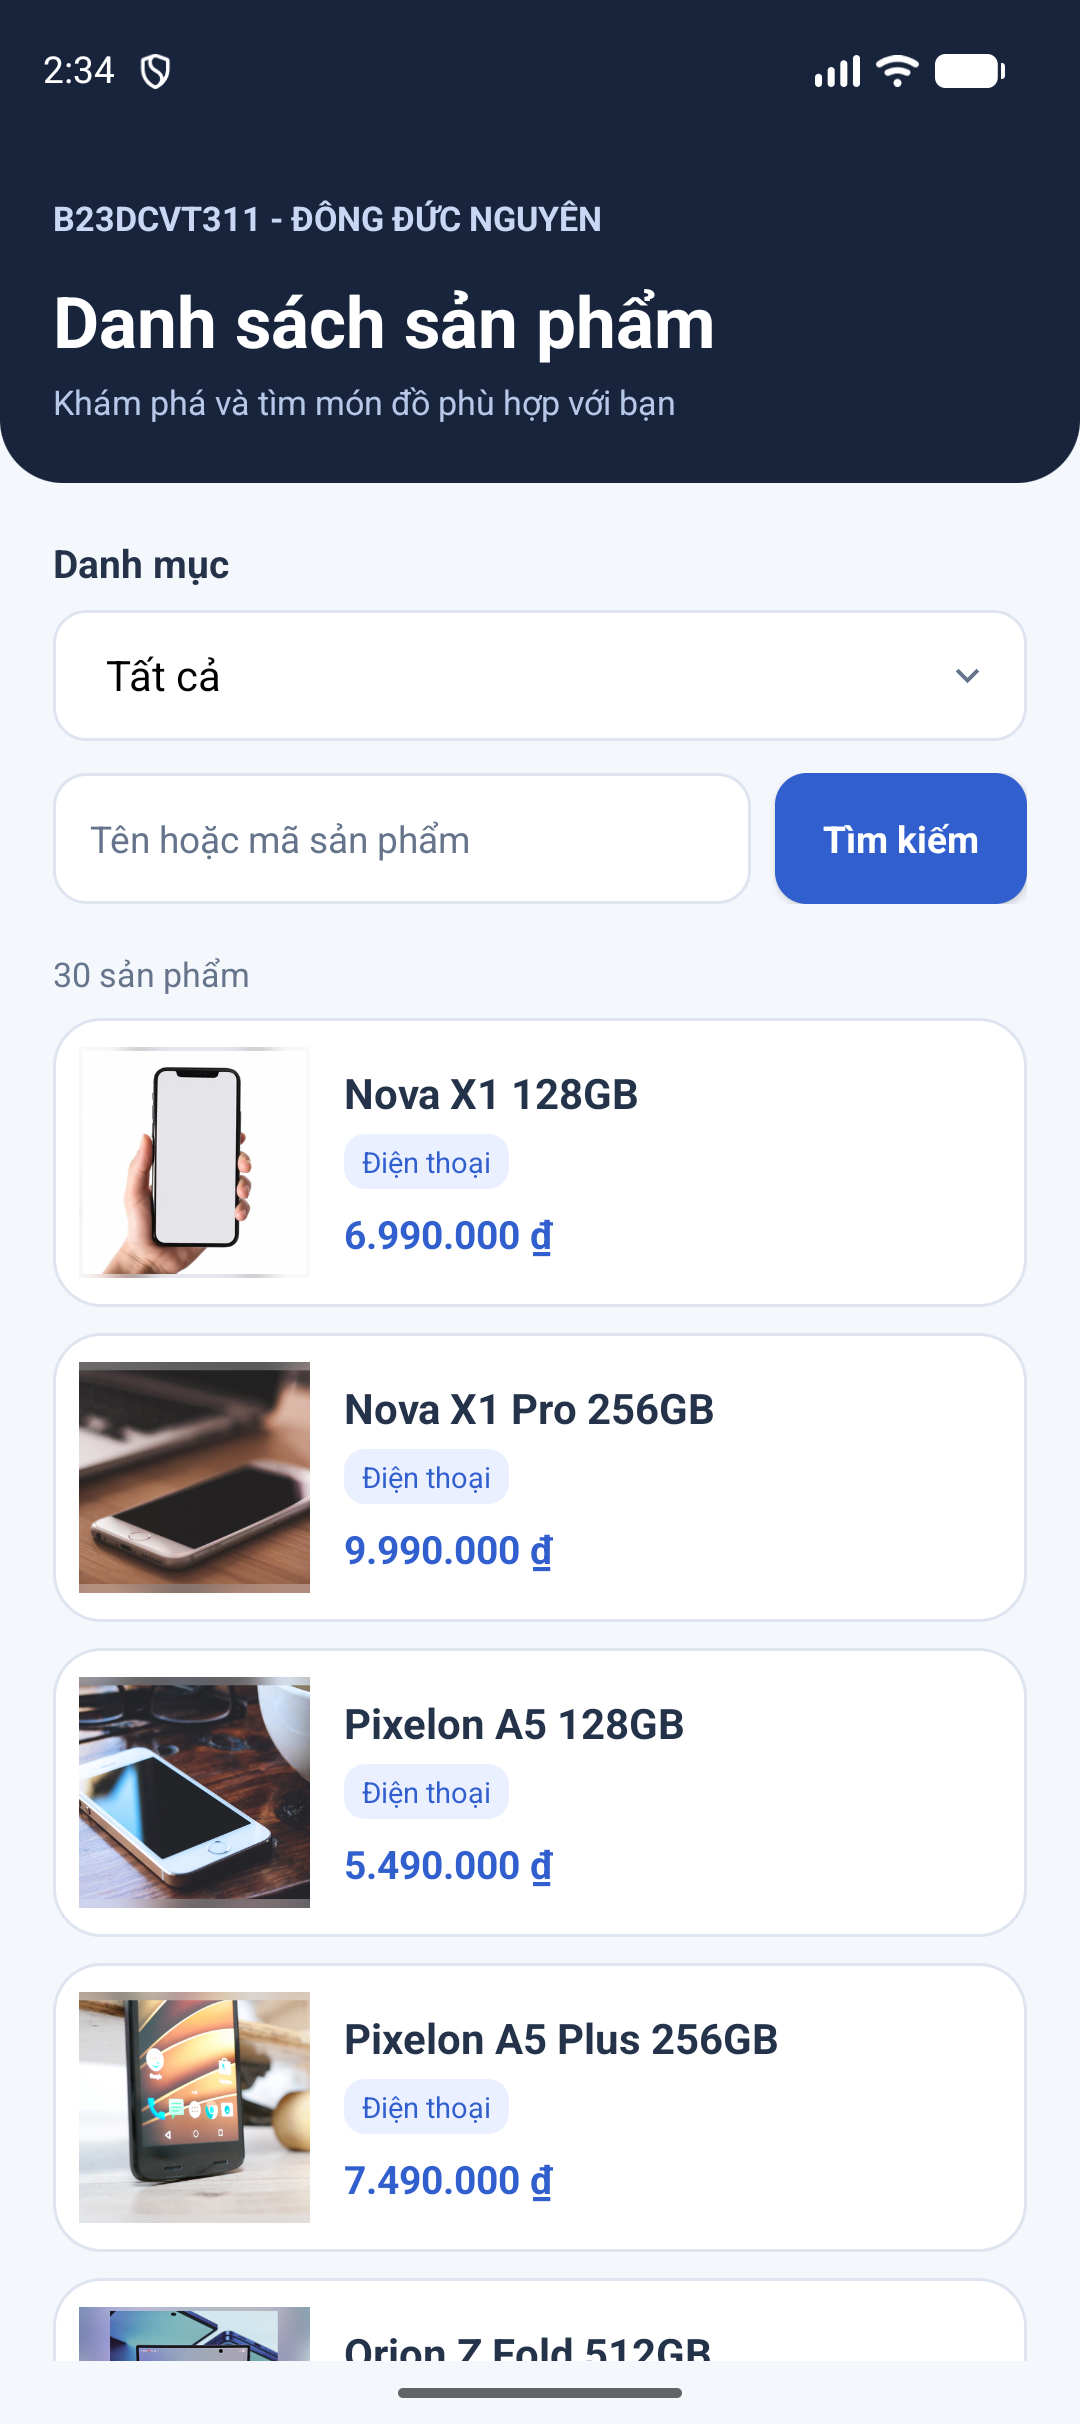
\includegraphics[width=0.86\linewidth]{01_main_activity.png}
\caption{Màn hình ban đầu: “Tất cả”, 30 sản phẩm.}
\label{fig:main}
\end{minipage}\hfill
\begin{minipage}[t]{0.46\textwidth}
\centering
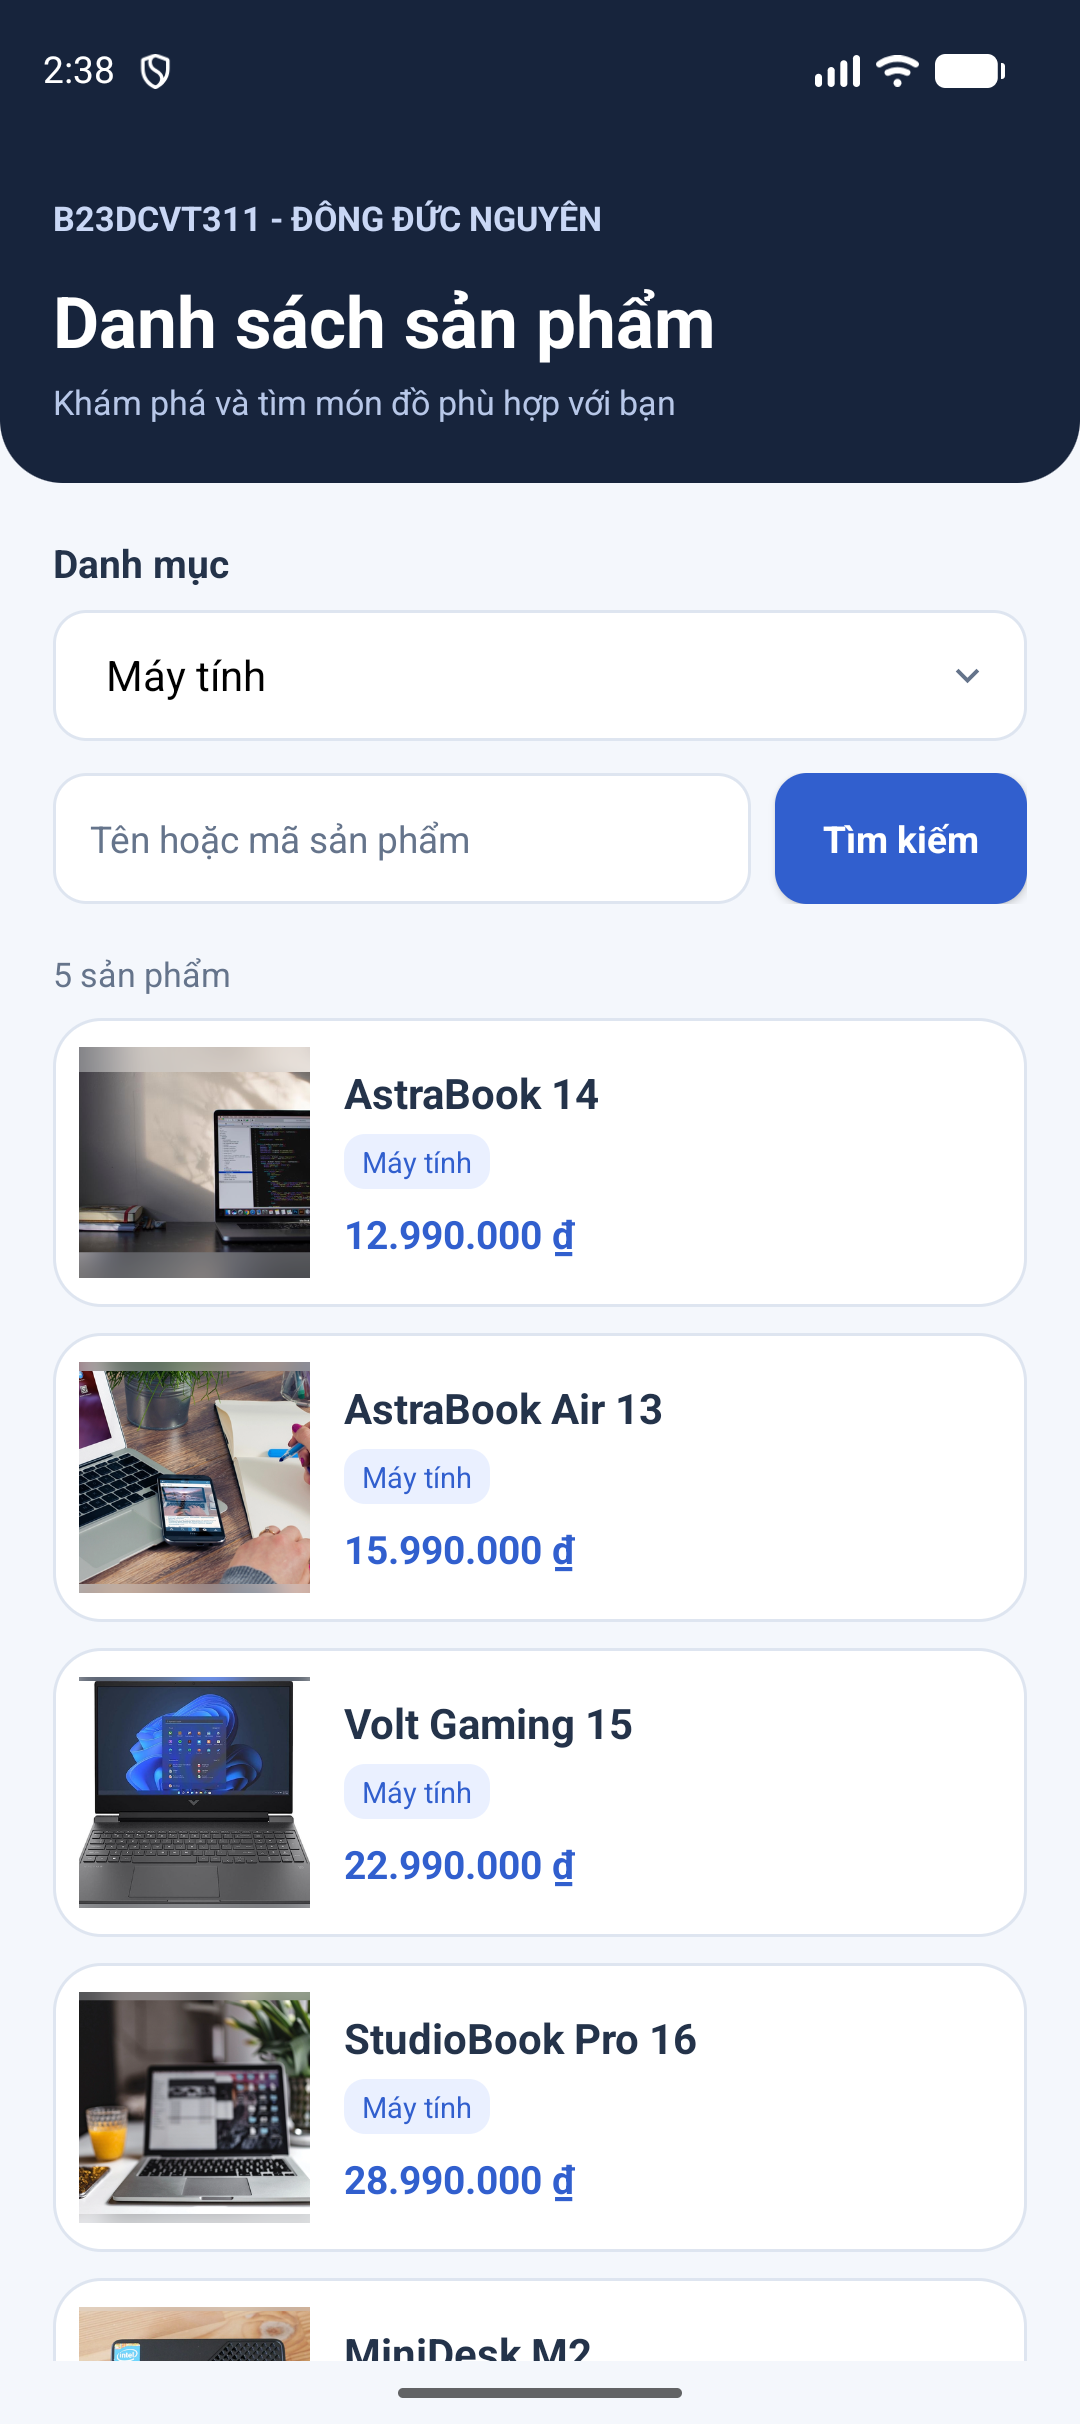
\includegraphics[width=0.86\linewidth]{02_filter_category.png}
\caption{Chọn “Máy tính”, còn 5 sản phẩm.}
\label{fig:filter}
\end{minipage}
\end{figure}
\noindent Hình~\ref{fig:main} cho thấy phần đầu của Activity, Spinner, bộ tìm kiếm,
nhãn tổng số 30 sản phẩm và các hàng có ảnh, tên, danh mục, giá.
Hình~\ref{fig:filter} cho thấy Spinner đã chọn “Máy tính” và danh sách
đúng 5 sản phẩm thuộc nhóm này.

\subsection{Tìm kiếm có kết quả và không có kết quả}
\begin{figure}[H]
\centering
\begin{minipage}[t]{0.46\textwidth}
\centering
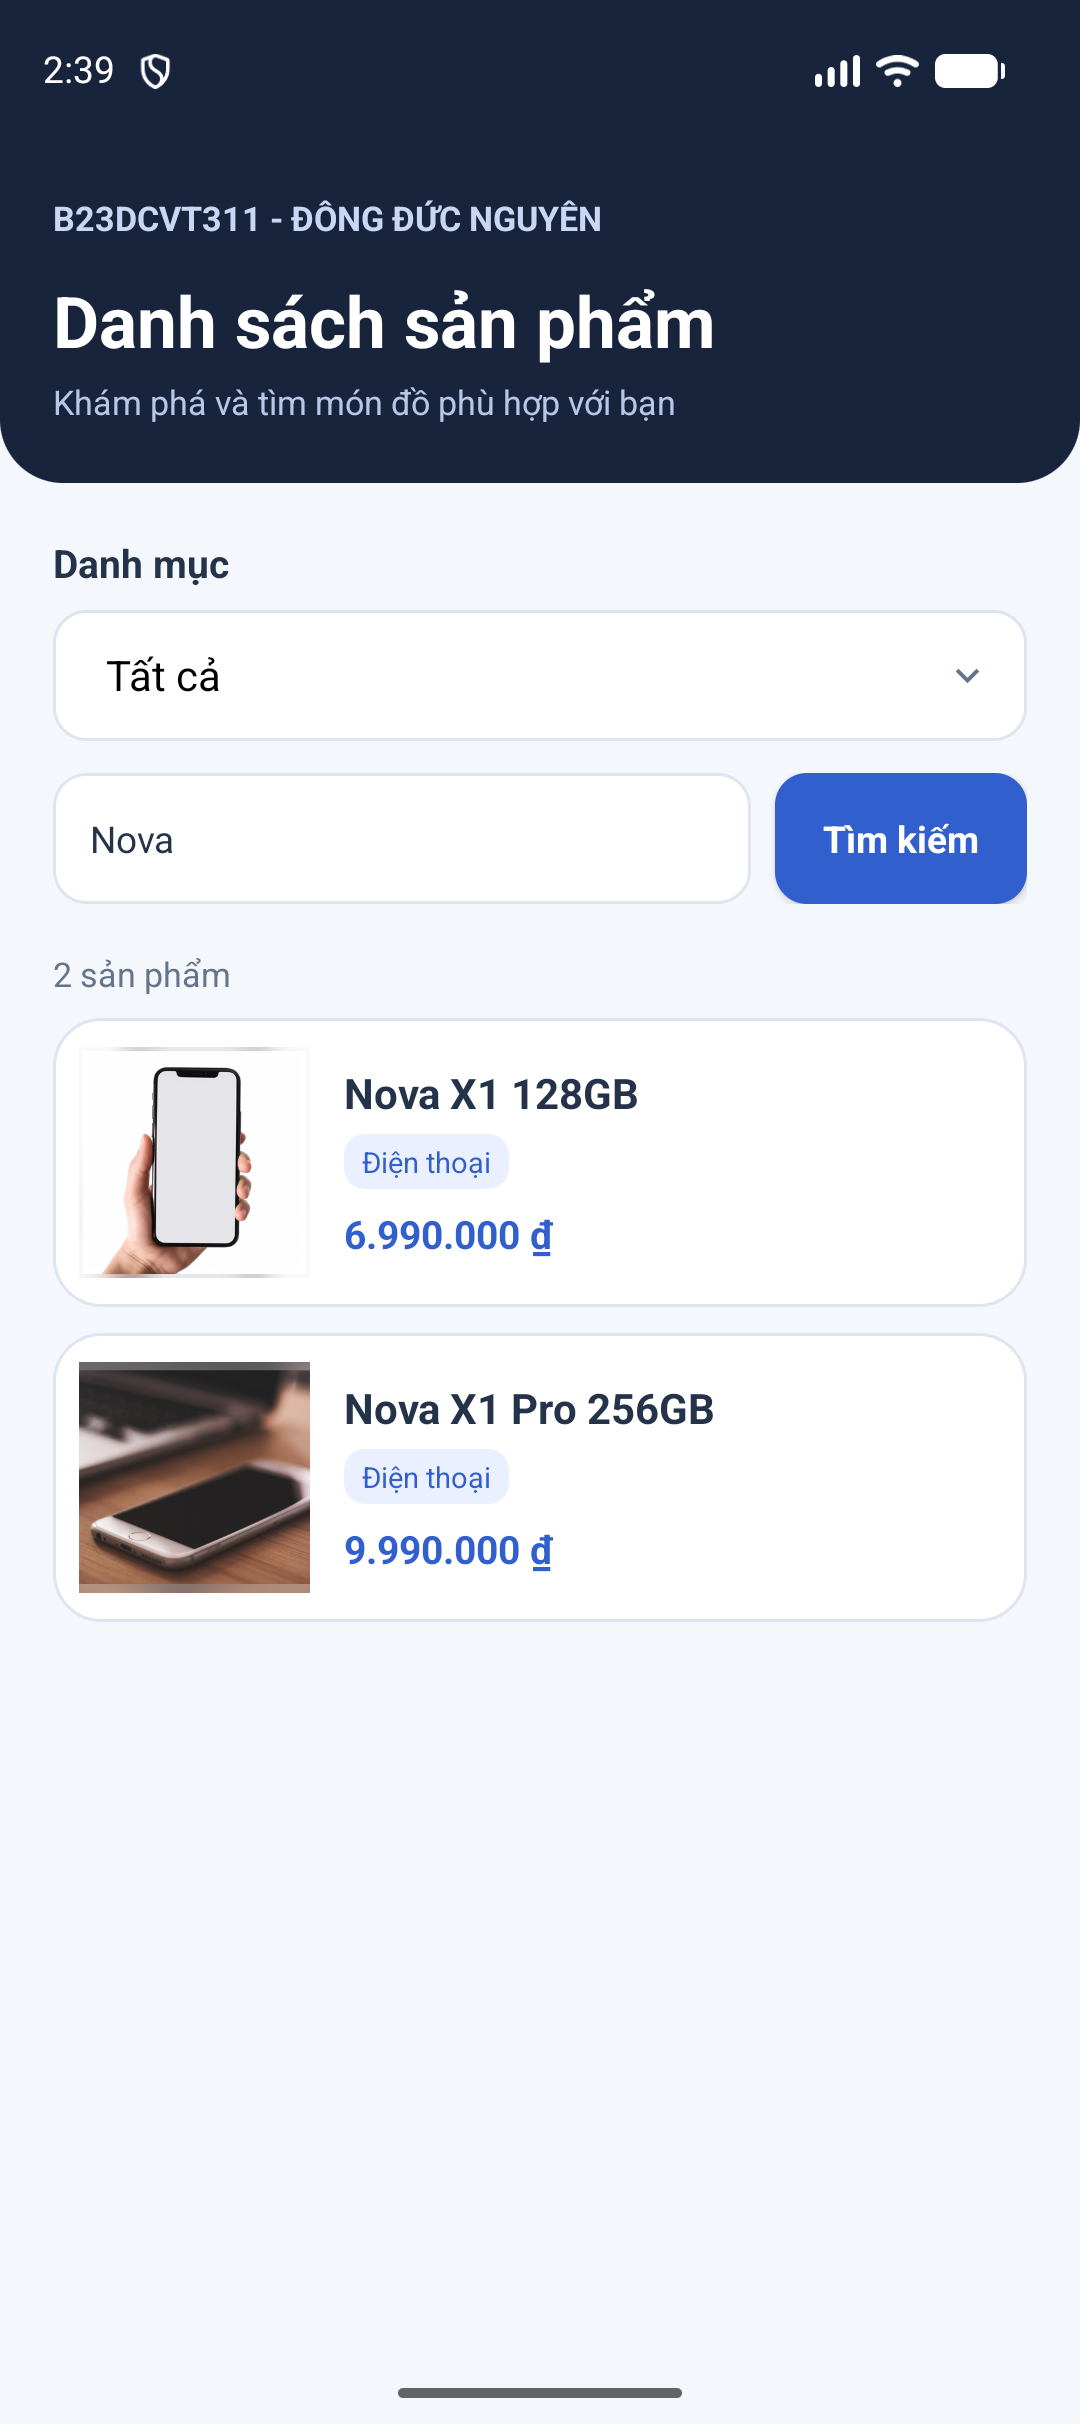
\includegraphics[width=0.86\linewidth]{03_search_product.png}
\caption{Tìm “Nova” trên toàn bộ sản phẩm: 2 kết quả.}
\label{fig:search}
\end{minipage}\hfill
\begin{minipage}[t]{0.46\textwidth}
\centering
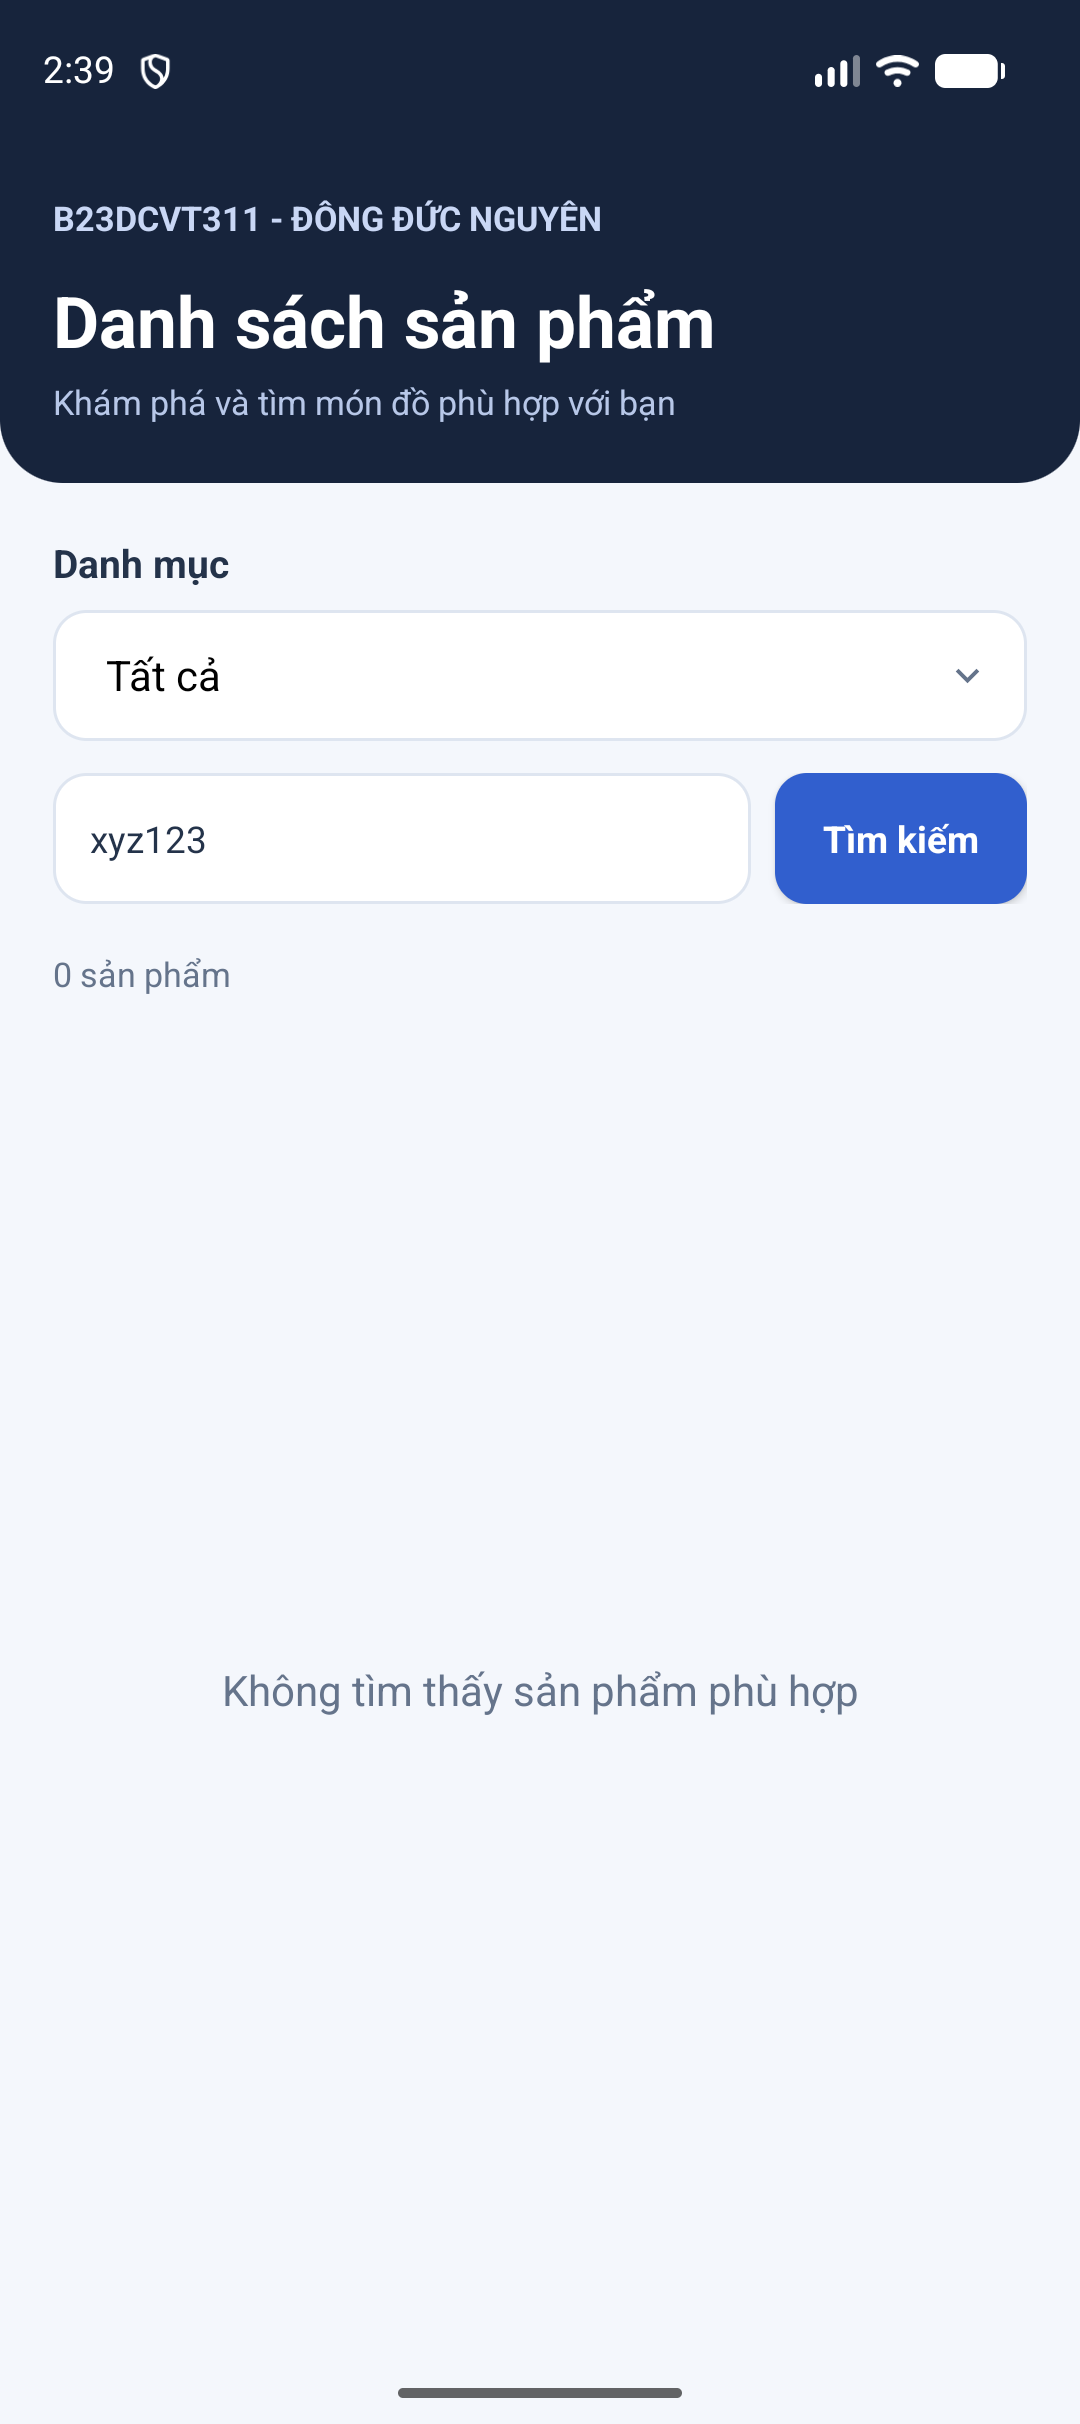
\includegraphics[width=0.86\linewidth]{04_search_no_result.png}
\caption{Tìm “xyz123”: 0 kết quả và thông báo rỗng.}
\label{fig:empty}
\end{minipage}
\end{figure}
\noindent Hình~\ref{fig:search} thể hiện truy vấn “Nova” cho hai sản phẩm điện thoại;
Spinner trở về “Tất cả”, phù hợp yêu cầu tìm kiếm độc lập với danh mục.
Hình~\ref{fig:empty} chứng minh trạng thái không có kết quả vẫn có phản hồi rõ ràng.

\subsection{Màn hình chi tiết sản phẩm}
\begin{figure}[H]
\centering
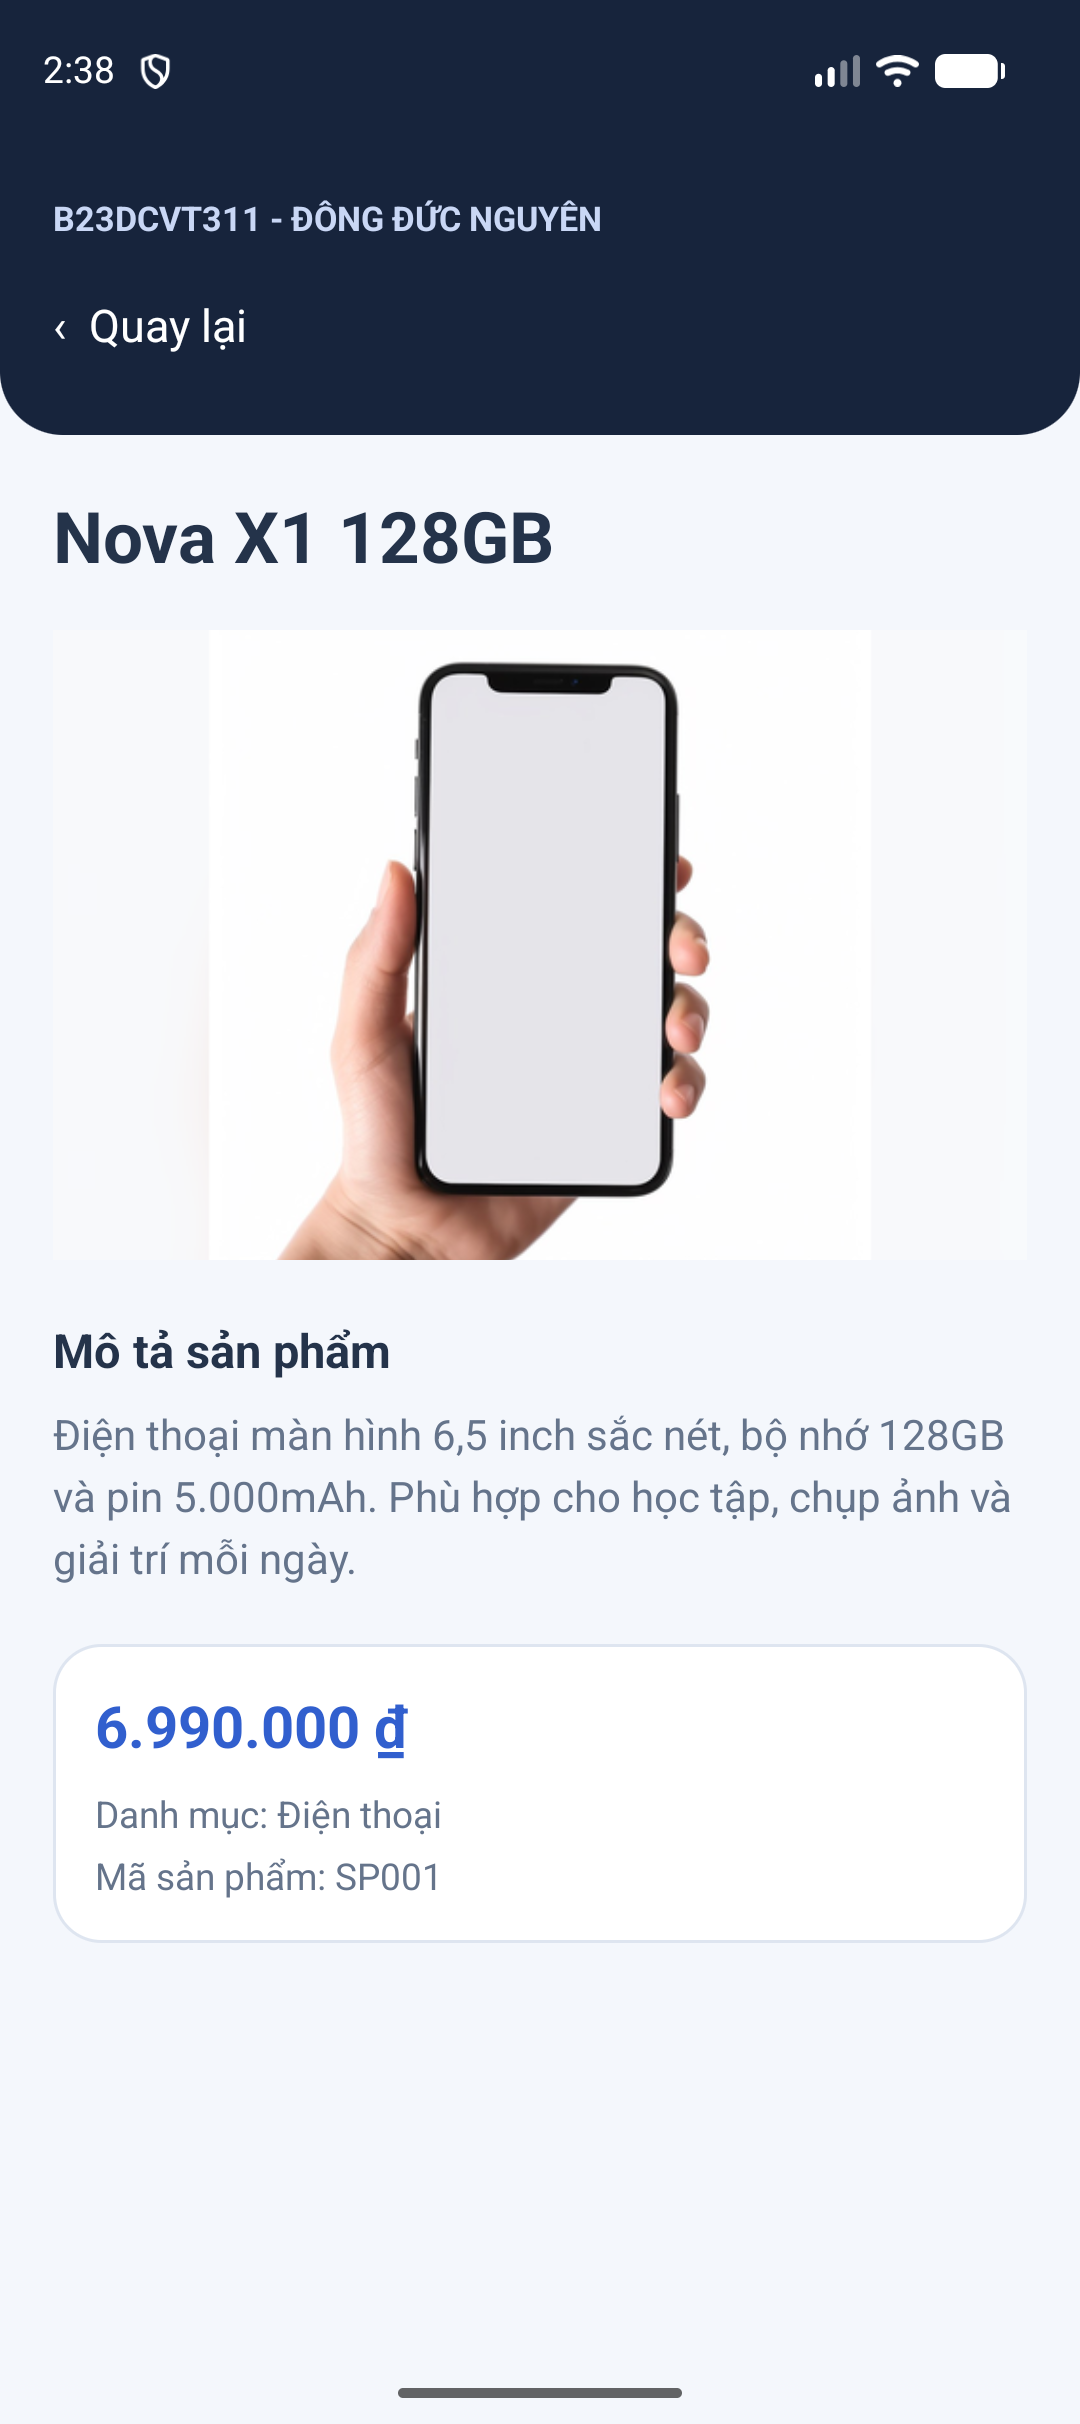
\includegraphics[width=0.42\textwidth]{05_product_detail.png}
\caption{Chi tiết sản phẩm \texttt{SP001}: tên, ảnh, mô tả và thông tin bổ sung.}
\label{fig:detail}
\end{figure}
\noindent Hình~\ref{fig:detail} cho thấy Activity thứ hai hiển thị sản phẩm
“Nova X1 128GB”, ảnh minh họa, mô tả, giá \texttt{6.990.000 đ},
danh mục “Điện thoại” và mã \texttt{SP001}. Phần đầu vẫn có thông tin sinh viên
và nút “Quay lại”.

\section{Kiểm thử và đánh giá}
\subsection{Môi trường}
Dự án dùng Kotlin, Android Gradle Plugin, \texttt{compileSdk = 35},
\texttt{minSdk = 23}, \texttt{targetSdk = 34} và JDK 17.
Lệnh \texttt{assembleDebug} tạo được APK ở
\codepath{app/build/outputs/apk/debug/app-debug.apk}.
Thiết bị giả lập đang dùng có độ phân giải 1080 $\times$ 2424.

\subsection{Các trường hợp kiểm tra}
\begin{table}[H]
\centering
\caption{Kịch bản và kết quả quan sát}
\small
\begin{tabularx}{\textwidth}{@{}p{0.9cm}p{3.9cm}X p{2.7cm}@{}}
\toprule
\textbf{STT} & \textbf{Thao tác} & \textbf{Kết quả mong đợi và quan sát} & \textbf{Minh chứng}\\
\midrule
1 & Mở ứng dụng & Hiện 30 sản phẩm; Spinner ở “Tất cả”. & Hình~\ref{fig:main}\\
2 & Chọn “Máy tính” & Hiện 5 sản phẩm của danh mục. & Hình~\ref{fig:filter}\\
3 & Tìm “Nova” & Spinner về “Tất cả”; hiện 2 kết quả. & Hình~\ref{fig:search}\\
4 & Tìm “xyz123” & Hiện 0 sản phẩm và thông báo phù hợp. & Hình~\ref{fig:empty}\\
5 & Chọn \texttt{SP001} & Chi tiết có đúng tên, ảnh, mô tả và giá. & Hình~\ref{fig:detail}\\
\bottomrule
\end{tabularx}
\end{table}
\noindent Kiểm tra dữ liệu cho thấy 30 bản ghi có mã riêng biệt, đủ sáu trường
theo thiết kế và cả 30 đường dẫn ảnh đều trỏ đến tệp hiện có.
Các trường hợp trong bảng đối chiếu hành vi giao diện với ảnh chụp thực tế.

\subsection{Điểm đạt được và giới hạn}
\begin{itemize}
\item Dữ liệu sản phẩm được đặt trong một tệp JSON; danh mục được suy ra từ dữ liệu,
tránh nhập danh sách danh mục lần thứ hai trong mã Activity.
\item Tìm kiếm dùng danh sách gốc, nên không chịu ảnh hưởng của lựa chọn Spinner trước đó.
Giao diện có phản hồi khi kết quả rỗng.
\item Ảnh được đóng gói cục bộ và có bộ đệm. Ứng dụng hoạt động ngoại tuyến.
\item Vì JSON và ảnh là tệp trong APK, thay đổi dữ liệu hoặc ảnh yêu cầu tạo lại và cài lại ứng dụng.
Tên mẫu sản phẩm trong bài là tên giả định; ảnh chụp CC0 đại diện đúng loại sản phẩm,
không phải ảnh xác thực của một mẫu thương mại cùng tên. Thông tin nguồn và giấy phép
được lưu trong metadata của từng PNG.
\end{itemize}

\section{Kết luận}
Bài thực hành đã triển khai đầy đủ chuỗi xử lý:
đọc JSON $\rightarrow$ tạo \texttt{ArrayList<Product>} $\rightarrow$
hiển thị bằng \texttt{ArrayAdapter<Product>} và \texttt{ListView} $\rightarrow$
lọc và tìm kiếm $\rightarrow$ mở Activity chi tiết.
Năm ảnh chụp màn hình minh chứng các trạng thái chính của ứng dụng.
Cấu trúc mã tách phần dữ liệu, ảnh, adapter và giao diện, thuận tiện cho việc
mở rộng thêm sản phẩm hoặc thay đổi bố cục về sau.

\appendix
\section{Hướng dẫn biên dịch và mở báo cáo}
\subsection{Ứng dụng Android}
Mở thư mục gốc bằng Android Studio và chạy cấu hình \texttt{app},
hoặc chạy \texttt{gradlew.bat :app:assembleDebug} trên Windows.
APK debug được đặt tại \codepath{app/build/outputs/apk/debug/app-debug.apk}.

\subsection{Báo cáo LaTeX}
Biên dịch \codepath{report/bao_cao_san_pham.tex} bằng XeLaTeX hoặc Tectonic
từ chính thư mục \codepath{report/}. Báo cáo sử dụng các ảnh trong
\codepath{report/figures/}. Phông chính là Times New Roman; phông mã là Consolas.
Các đoạn mã trong báo cáo tập trung vào những phần triển khai chức năng,
còn mã nguồn đầy đủ nằm trong thư mục \codepath{app/src/main/}.

\end{document}
